\chapter{Introduction to QGIS (using v3.14)}

\pagestyle{fancy}
\fancyhf{}
\fancyhead[OC]{\leftmark}
\fancyhead[EC]{\rightmark}
%\renewcommand{\footrulewidth}{1pt}
\cfoot{\thepage}

%%%%%%%%%%%%%%%%%%%%%%%%%%%%%%%%%%%%%%%%%%%%%%%%%%%%%%%%%%%
%%%%%%%%%%%%%%%%%%%%%%%%%%%%%%%%%%%%%%%%%%%%%%%%%%%%%%%%%%%

\section{Online resources}

QGIS tutorials: \url{https://docs.qgis.org/3.4/en/docs/} \\
Online forums:  \url{https://stackexchange.com/} \\

\section{This tutorial}

\subsection{We will cover these QGIS skills}
\begin{enumerate}[~~~1)]
%\begin{itemize}[noitemsep]
%\begin{compactitem}[$\bullet$]
	\item
	Introduction to the QGIS software environment
	\item
	Loading data into QGIS
	\item
	Viewing spatial data (with and without geometry fields)
	\item
	Adding symbology
	\item
	Using a base map
	\item
	Brief introduction to using expressions
	\item
	Creating print layout
%\end{itemize}
\end{enumerate}
%\end{compactitem}

%\begin{itemize}[noitemsep,nolistsep]

\subsection{Tutorial data}
The tutorial's example is based on data for the five forces in the SW England (Devon \& Cornwall, Avon \& Somerset, Wiltshire, Gloucestershire, Dorset) for three years (September 2016 - August 2019). Data for this tutorial was downloaded from \url{ https://data.police.uk/data}
and edited to be in a usable format. QGIS can use many types of data, including raster and vector layers. In this tutorial we will only use vector data.\\

\null\newpage

This tutorial will use 4 data files:
\begin{enumerate}[~~~1)]
	\item
	\textbf{Shapefile} containing the visual boundaries of the LSOA polygons for the counties covered by the five forces\\
	$LSOA\_2011\_sw5forces\_BGC\_V2.shp$
	\item
	\textbf{CSV file without geometry fields} containing crime type (count) from each LSOA\\
	$sw\_5forces\_street\_by\_lsoa.csv$
	\item
	\textbf{CSV file with geometry fields} containing location of stop and searches\\
	$sw\_5forces\_stop\_and\_search.csv$
	\item 
	\textbf{CSV file with geometry fields} containing the location of police headquarters\\
	$headquarters.csv$
\end{enumerate}

Using these files, we will produce maps to visually represent the:
\begin{enumerate}[~~~1)]
	\item
	number of crimes per Lower Super Output Area (LSOA)
	\item
	locations of stop and search incidences
	\item
	locations of Police headquarters
\end{enumerate}

Below is an example of a map showing data for items \#1 and \#3 above.
\begin{figure}[!h]
	\centering
	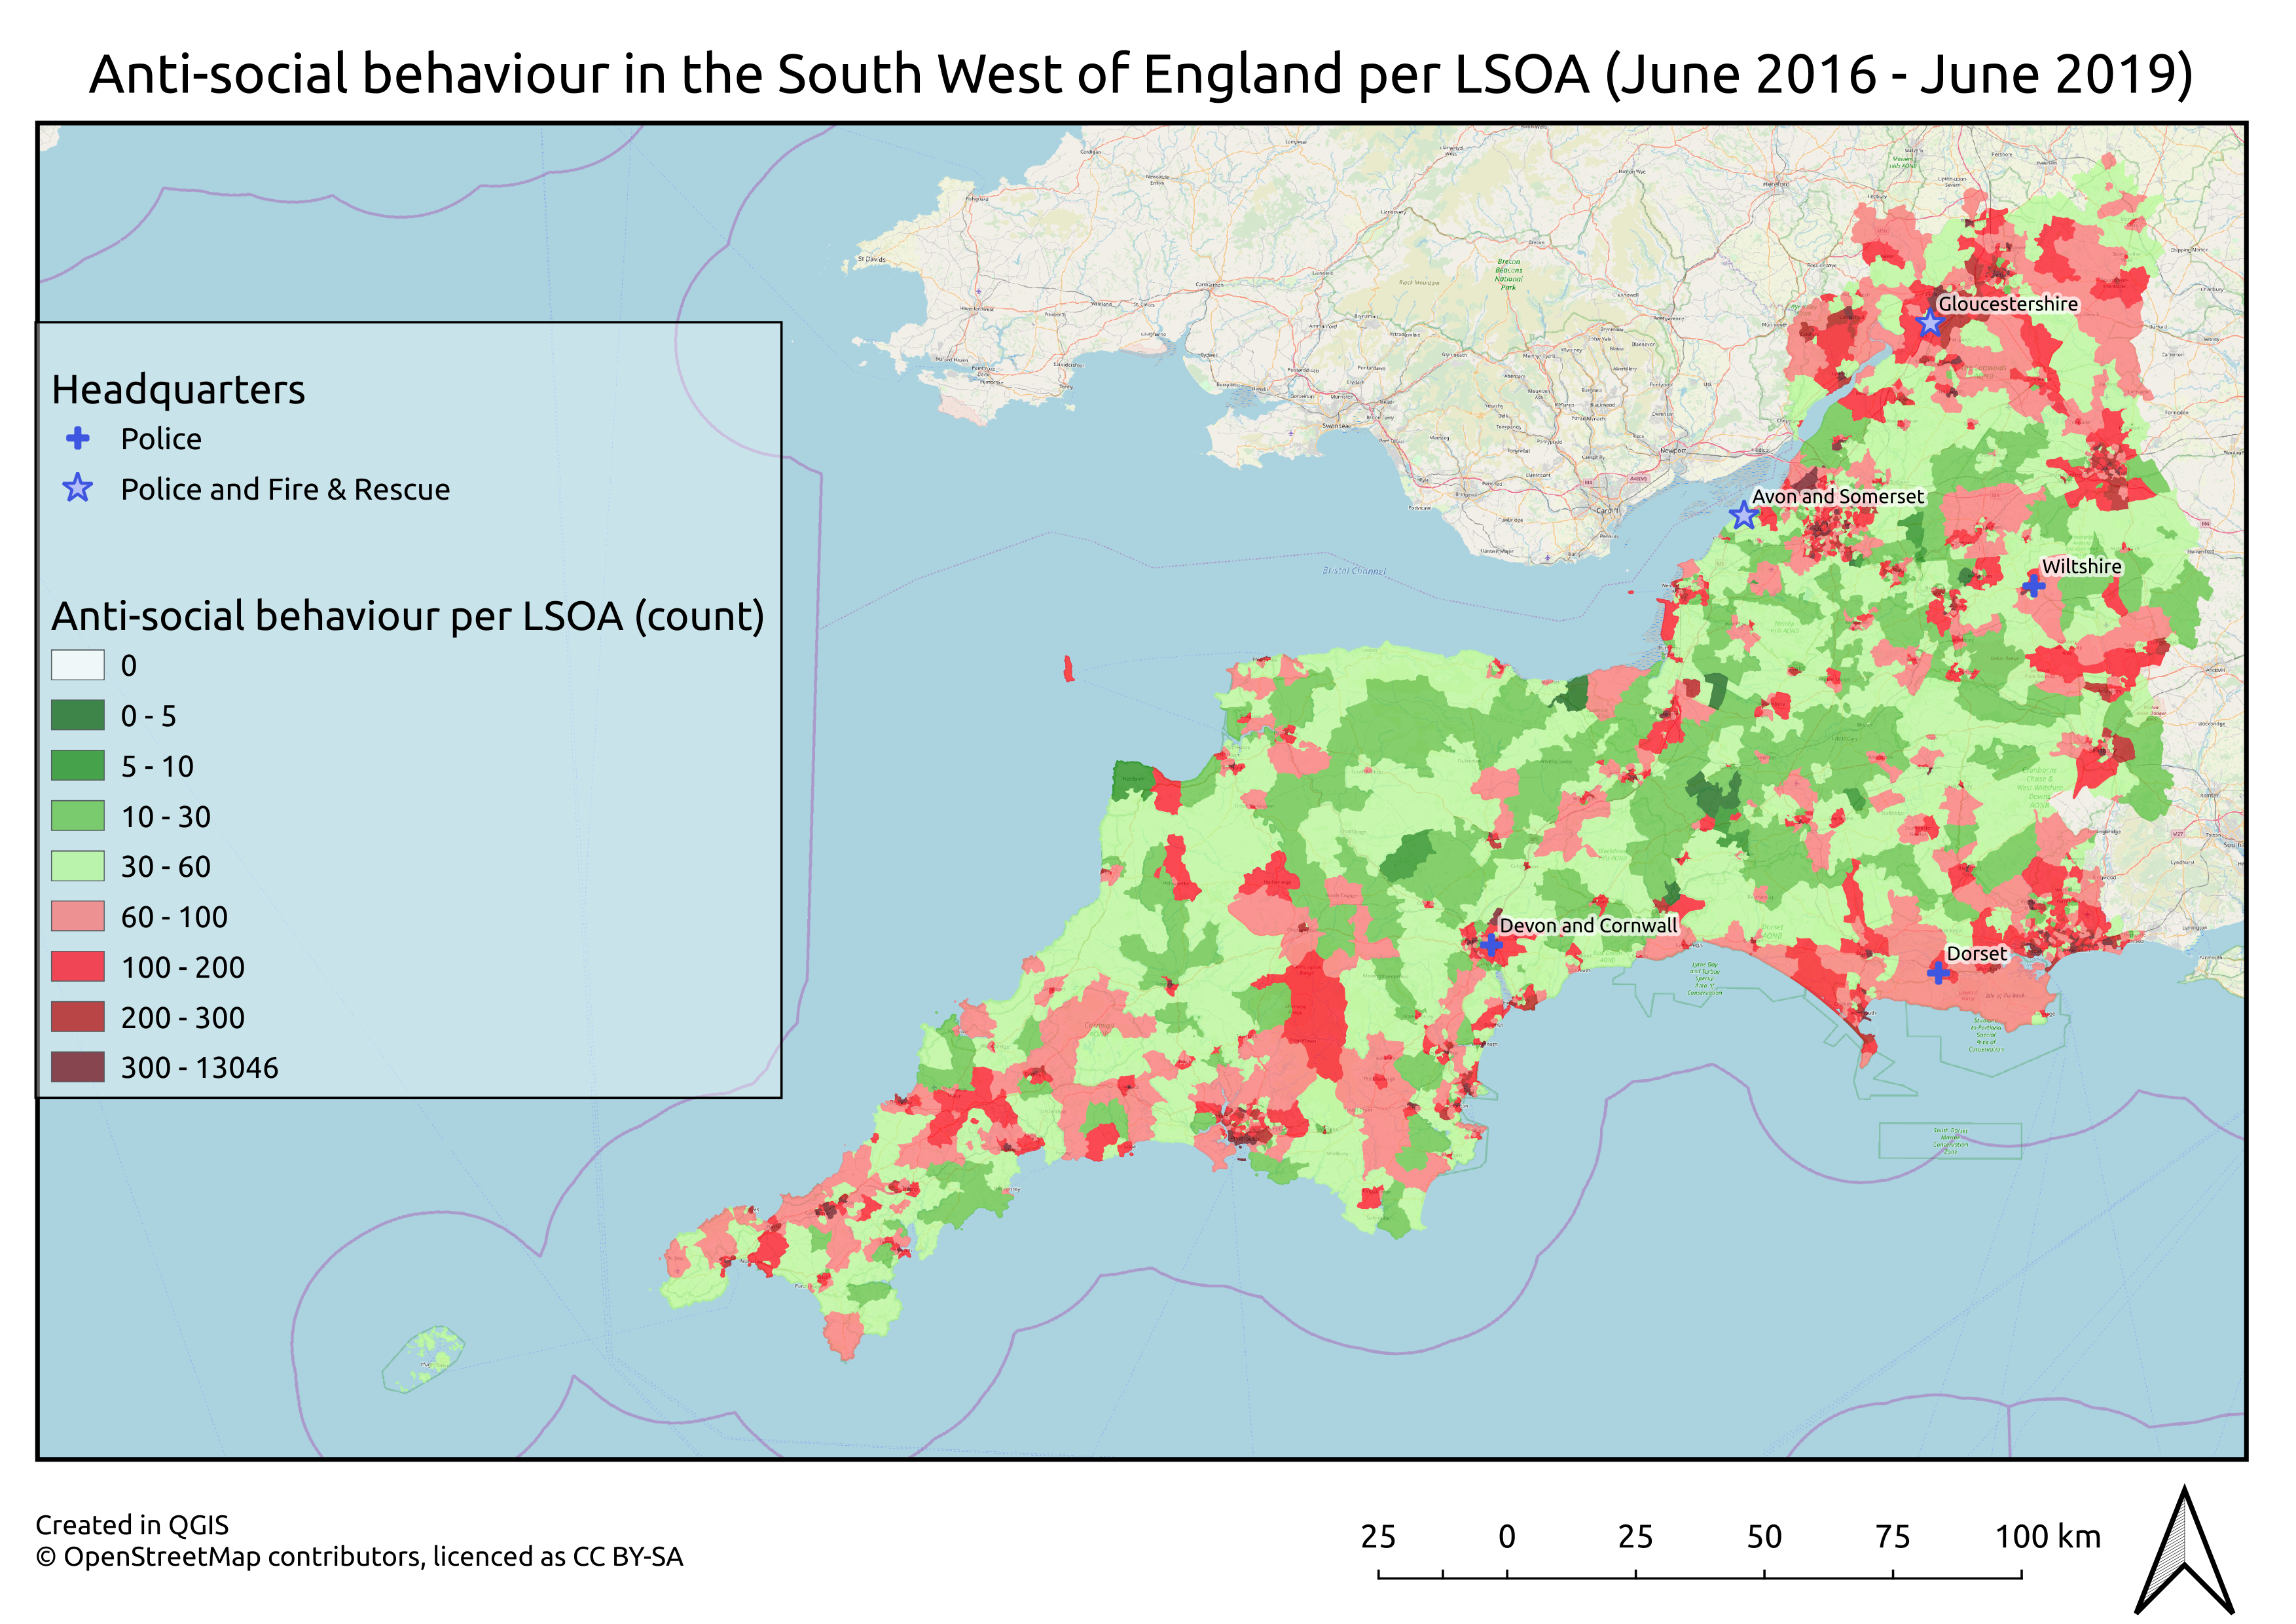
\includegraphics[width=0.9\textwidth]{images/headquarter_crime_map.png}
	\caption{An example of a map we will create in this tutorial. Using QGIS, LSOA shapefile, and own data in csv files}
	\label{ft_fig_firstfig3}
\end{figure}


